\documentclass[journal]{IEEEtran}
\usepackage{amsmath}
\usepackage{graphicx}
\usepackage{biblatex}

\usepackage{biblatex}
\addbibresource{referencias.bib} %Imports bibliography file

\def\BibTeX{{\rm B\kern-.05em{\sc i\kern-.025em b}\kern-.08em
    T\kern-.1667em\lower.7ex\hbox{E}\kern-.125emX}}


\usepackage{hyperref}
\hypersetup{
    colorlinks=true,
    linkcolor=blue,
    filecolor=magenta,      
    urlcolor=cyan,
}

\usepackage[portuguese]{babel}
\usepackage{hyphenat}
 
 
\urlstyle{same}

\begin{document}
%TITULO DO TRABALHO
\title{Desenvolvimento de Projeto - Laboratório de Projetos VI}

%AUTOR DO TRABALHO
\author{\IEEEauthorblockN{Felipe Fonseca Rocha}
\IEEEauthorblockA{\textit{2015096117} 
feliperocha@ufmg.br\\}
\and
\IEEEauthorblockN{Isaac Henrique Simões}
\IEEEauthorblockA{\textit{2015435713} 
caasihenrique@ufmg.br\\}
\and
\IEEEauthorblockN{Renata M. R. Nésio}
\IEEEauthorblockA{\textit{2014140418} 
renatanesio@ufmg.br\\}
\and
\IEEEauthorblockN{Tiago Lobato Mansur}
\IEEEauthorblockA{\textit{2014016059} 
lobat@ufmg.br}}


%NEGRITO E RODAPES ETC
\markboth{Desenvolvimento de Projeto - Laboratório de Projetos VI,~2º semestre 2020, No.~11,~Dezembro~2020}%
% {Shell \MakeLowercase{\textit{et al.}}: Modelagem de um problema prático simples e solução do problema de otimização
% aplicando técnicas e conceitos de otimização}

%INSERE O TÍTULO
\maketitle

%RESUMO
\begin{abstract}

A Ogranização Mundal da Saúde (OMS) junto a governos de diversos países
\end{abstract}

\begin{IEEEkeywords}
análise de dados temporal, doenças respiratórias, distribuição econômica, .
\end{IEEEkeywords}

\IEEEpeerreviewmaketitle

\section{Introdução}

\IEEEPARstart{A} {Organização} Mundial da Saúde (OMS) lançou a Aliança Global contra Doenças Respiratórias (GARD) em 2006 com o objetivo de reunir o conhecimento combinado de organizações, instituições e agências nacionais e internacionais para melhorar a vida de mais de um bilhão de pessoas afetadas por doenças crônicas e doenças respiratórias agudas\cite{firs}.

Em 2015 líderes mundiais adotaram a Agenda de Desenvolvimento Sustentável 2030 proposta pela Organização das Nações Unidas. O terceiro objetivo da Agenda é "garantir vidas saudáveis e promover o bem-estar para todos em todas as idades". A organização defende que a melhoria da saúde tirará as pessoas da pobreza e contribuirá substancialmente para o desenvolvimento da sustentabilidade.

Também na Organização das Nações Unidas existe um esforço para dar importância a temas correlatos, sendo o terceiro objetivo de desenvolvimento sustentável, assegurar uma vida saudável e promover o bem-estar a todos em qualquer idade.

A OMS define como doenças respiratórias as doenças ou infecções que ocorrem no trato respiratório, tanto das vias superiores,fossas nasais, faringe e laringe, como inferior, traqueia, os pulmões, os brônquios, os bronquíolos e os alvéolos pulmonares em que há a obstrução da circulação do ar.

Apesar das infecções das vias respiratórias superiores, como por exemplo faringite e laringite, sejam muito recorrentes, mas raramente com risco  de vida, as infecções das vias respiratórias inferiores (IVRI) são responsáveis por doenças mais graves contribuindo para mortalidade por infecções respiratórias agudas (IRAs).

As Síndrome Respiratória Aguda Grave (SRAG) são definidas quando o indivíduo hospitalizado com febre, mesmo que referida, acompanhada de tosse ou dor de garganta e que apresente dispneia ou saturação de O2 menor que 95\% ou desconforto respiratório ou que evoluiu para óbito por SRAG independente de internação \cite{definicao}.

De acordo como a OMS, as IRAs estão entre as doenças infecciosas de maior índice de morbimortalidade em todo o mundo, afetando o público infantil e os mais idosos. Essas infecções são, geralmente causadas por vírus, podendo também ser causadas por bactérias.

As doenças respiratórias na infância têm constituído a cada dia motivo de preocupação para os profissionais de saúde, dada a sua elevada morbidade, observada em termos mundiais, bem como a alta mortalidade que incide especialmente nos países do terceiro mundo. Segundo dados divulgados pela Organização Mundial da Saúde (OMS), cerca de 13 milhões de crianças menores de cinco anos morrem anualmente no mundo por doenças do aparelho respiratório e 95\% delas ocorrem nos países em desenvolvimento \cite{infantil}.

Na faixa etária de seis meses aos três anos, as crianças têm de seis a nove infecções respiratórias agudas por ano, sendo que  cerca  de  10\%  delas  apresentam  mais  de  dez  quadros  ao  ano.  Entre  os  três  e  cinco  anos,  o  número  de  infecções  respiratórias cai para três a quatro por ano, e crianças acima dos cinco anos apresentam um a dois quadros por ano, como ocorre nos adultos. Esse é um comportamento fisiológico decorrente do desenvolvimento do sistema imunológico \cite{infeccao}.

As doenças respiratórias são altamente contagiosas devido ao seu elevado potencial de propagação através da projeção de gotículas contaminadas durante a fala, espirro, tosse e bocejo.  O contato da mão com superfícies contaminadas e em seguida a auto inoculação com essa constitui a principal via de transmissão.

A relevância da saúde das populações têm relação direta com a qualidade de vida dessa população \cite{sdgsonu}, bem como a sustentabilidade de atividades econômicas desenvolvidas, sem falar no impacto orçamentário para divisão de saúde pública, do tratamento de doenças respiratórias agudas, 5,9\% dos registos de internação do ano de 2019\cite{ansdoencarespiratoria} são dessa categoria de doença.

Sabendo que algumas infecções respiratórias das vias aéreas superiores são causadas por vírus sazonais, mais frequentes no período frio em áreas de clima temperado e também no período de chuvas naquelas de clima tropical\cite{azevedo_santos_silva_olinda_santos_2017}, este trabalho busca correlacionar condições climáticas a casos de doenças respiratórias.

Sabendo da necessidade de desenvolvimento contínuo de avaliação dos dados e a natureza efêmera de modelos pela rápida alteração do contexto em que são desenvolvidos, vide o último ano (2020). Precisamos encontrar métodos de atualização contínua desses modelos e também um controle de contexto (base de dados e parâmetros) utilizados durante a análise. Também é necessário que esse método comporte a gestão de complexidade inerente ao desenvolvimento de múltiplos modelos, onde provavelmente o modelo que descrevia a temporalidade e possíveis relações econômicas e meteorológicas das doenças respiratórias em 2019, não se aplica a 2020, sendo a COVID-19 um evento não mapeado anteriormente produzindo novos comportamentos entre os componentes do sistema modelado.

% %RODAPE DA INTRODUÇÃO
% \hfill Felipe Fonseca Rocha
 
% \hfill 11 de Dezembro de 2020

\section{Proposta}

\subsection{Objetivos}

\emph{Utilizar} uma metodologia de processamento de dados automatizado (conhecido como \emph{MLOps}) para dados em saúde pública afim de entender a distribuição temporal de doenças respiratórias agudas sob perspectivas geoclimáticas com dados encontrados no Banco de Dados Meteorológicos do Instituto Nacional de Meteorologia\cite{bdmep_2020} e socioeconômicas, com dados extraídos do Portal de Transparência do Governo Federal \cite{PortalTransparência2020}.

\subsubsection{Gerais}
O projeto busca produzir um artefato de software ou uma plataforma automatizada de processamento de dados de saúde pública advindo da base de dados do SUS disponibilizada no Portal Brasileiro de Dados Abertos\cite{DadosGov}.


\subsubsection{Específicos}
Busca-se encontrar uma forma de transformar dados públicos em informação de baixo ou nenhum custo à população viabilizando seu acesso através de uma plataforma de alta disponibilidade aplicando as melhores práticas na esteira de processamento e tratamento dos dados diretos de banco.
\subsection{Originalidade do Projeto}
Atualmente existe uma grande volume de dados disponíveis sobre o sistema de saúde brasileiro. Saber como encontrá-los, o que procurar e como interpretá-los, no entanto, não é uma tarefa trivial. Dessa forma, a originalidade do projeto está na criação e disponibilização de um artefato para que qualquer cidadão em posse de um determinado dado possa então processá-lo e com isso obter informações e interpretá-las sem que um conhecimento de programação seja necessário.
\subsection{Análise do Problema Proposto}
O problema é a inexistência de uma apresentação dos dados do sistema de saúde brasileiro de forma simples, intuitiva e de fácil acesso a população, mesmo existindo um grande volume de dados disponível. Dessa forma, o desafio é conseguir centralizar estes dados, interpretá-los e relacioná-los com aspectos externos e apresentá-los de forma simples, intuitiva e acessível para todos. 
\subsection{Equipe}
\begin{itemize}
    \item Felipe Fonseca Rocha
    \item Isaac Henrique Simões
    \item Renata Nésio
    \item Tiago Lobato Mansur
\end{itemize}

\subsubsection{Habilidades}
\begin{itemize}
   \item Felipe Fonseca Rocha
   \begin{itemize}
     \item Desenvolvimento de software
     \item Arquitetura \textit{Cloud Computing}
     \item DevOps e infraestrutura
     \item Arquitetura de Software
   \end{itemize}

    \item Isaac Henrique Simões
    \begin{itemize}
        \item Análise de dados
        \item Modelagem de matemática
    \end{itemize}

    \item Renata Nésio
   \begin{itemize}
     \item Programação
     \item Machine learning 
     \item Gestão de projetos
     \item Análise de dados
   \end{itemize}

   \item Tiago Lobato Mansur
   \begin{itemize}
     \item Desenvolvimento de software
     \item Gestão de equipe
   \end{itemize}

\end{itemize}
\subsubsection{Responsabilidades}
\begin{itemize}
   \item Felipe Fonseca Rocha
   \begin{itemize}
     \item Aplicação da metodologia CML
     \item Gerenciamento de Infraestrutura
     \item Gerenciamento dos Pipelines
     \item Extração e limpeza dos dados
     \item Gerenciamento do repositório
     \item Automação de tarefas 
   \end{itemize}
   
   \item Isaac Henrique Simões
   \begin{itemize}
       \item Codificação
   \end{itemize}
   
    \item Renata Nésio
   \begin{itemize}
     \item Aplicação da metodologia CML
    \item Análise de dados obtidos
     \item Extração de dados
     \item Gestão do projeto
     \item Automação de tarefas 

   \end{itemize}
   
   \item Tiago Lobato Mansur
   \begin{itemize}
     \item Centralização e tradução dos dados
     \item Gestão da equipe
   \end{itemize}
\end{itemize}
\subsection{Analise de Viabilidade}

Para avaliar a viabilidade do projeto, foi elaborado um gráfico de Gantt, apresentado na Fig.\ref{fig:Gantt}.

\begin{figure}[htpb]
    \centering
    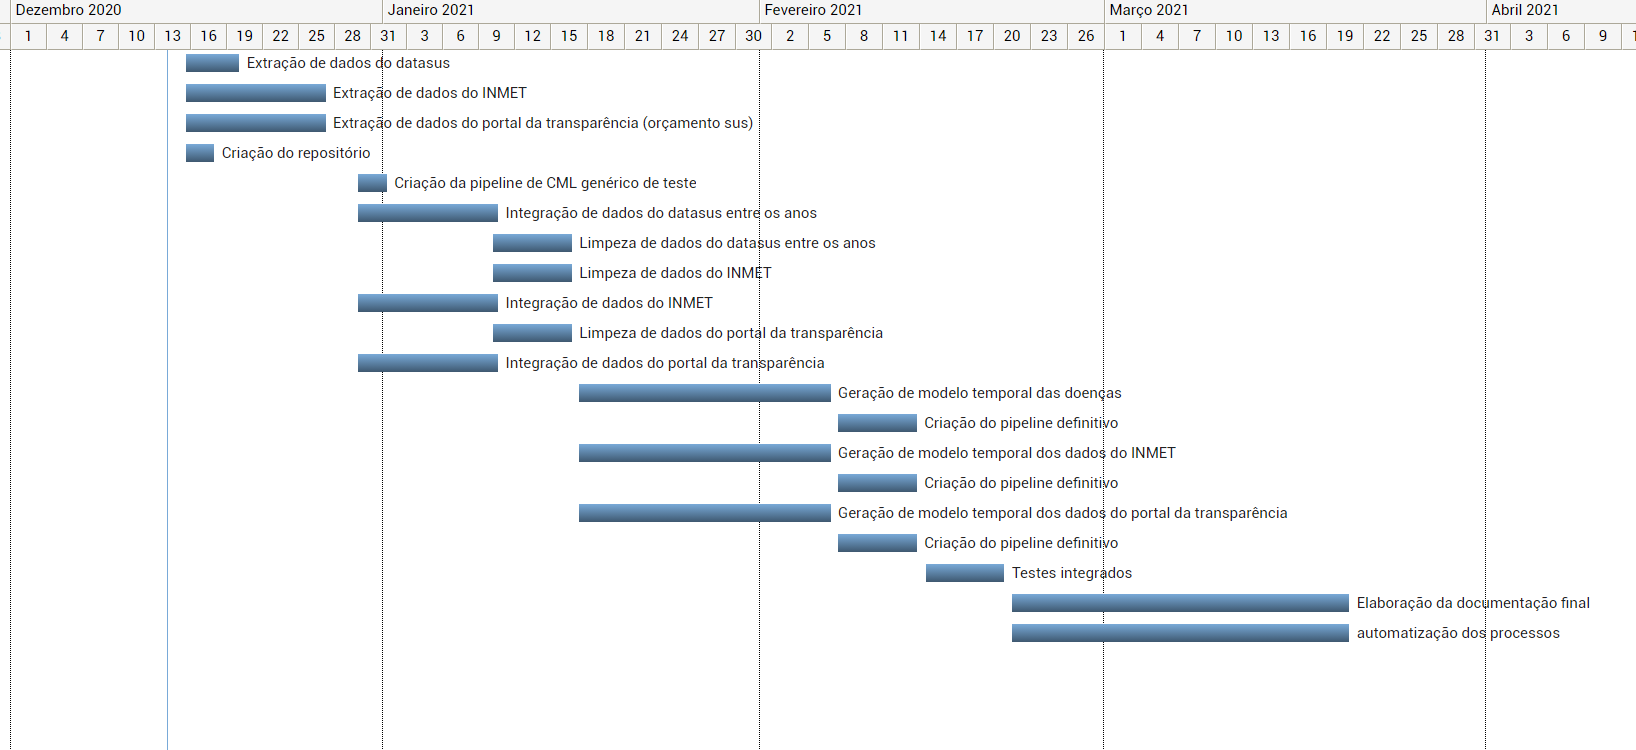
\includegraphics[height=4cm,keepaspectratio=true]{docs/Cronograma.PNG}
    \caption{Cronograma com gráfico de Gantt}
    \label{fig:Gantt}
    \centering
\end{figure}

Dados os prazos estabelecidos, que são, por ora, uma aproximação  do tempo necessário para cada tarefa, a realização das tarefas propostas parece viável até o momento.


\section{estudo de anterioridade} 
% ####################################
As doenças respiratórias juntamente com as cardiovasculares, cânceres e diabetes, são as doenças não transmissíveis (DNT) que mais matam hoje.
O Fórum das Sociedades Respiratórias Internacionais (FIRS) aborda a relação que existe nas doenças respiratórias e o meio ambiente. A queima de combustíveis, a poluição de fontes industriais e a fumaça do tabaco contribuem para a maioria das condições respiratórias \cite{firs}.

A infecção respiratória aguda do trato inferior é causa de aproximadamente 4 milhões de mortes por ano e são a principal causa de morte em crianças abaixo de 5 anos. É uma causa particularmente importante de morte em países de baixa e média renda. Entre as 30 causas mais comum de morte, a infecção é a quarta \cite{firs}.

As  doenças  respiratórias  são influenciadas por queimadas e os efeitos de inversões térmicas que concentram a poluição, impactando diretamente a qualidade do ar, principalmente nas áreas urbanas \cite{mudanças}.

A variação de respostas humanas relacionadas às mudanças  climáticas  parece  estar  diretamente  associada às  questões  de  vulnerabilidade  individual  e  coletiva. Variáveis  como  idade,  perfil  de  saúde,  resiliência  fisiológica e condições sociais contribuem diretamente para  as  respostas  humanas  relacionadas  às  variáveis climáticas.  Alguns  estudos também  apontam  que  alguns  fatores  que  aumentam a  vulnerabilidade  dos  problemas  climáticos  são  uma combinação  de  crescimento  populacional,  pobreza  e degradação  ambiental \cite{mudanças}.

As  condições  atmosféricas  podem  influenciar  o  transporte  de  microrganismos,  assim  como  de  poluentes oriundos de fontes fixas e móveis e a produção de pólen. Os efeitos das mudanças climáticas podem ser potencializados, dependendo das características físicas e químicas dos poluentes e das características climáticas como temperatura, umidade e precipitação. Essas características definem o tempo de residência dos poluentes na atmosfera, podendo ser transportados a  longas  distâncias  em  condições  favoráveis  de  altas temperaturas  e  baixa  umidade.  As alterações de temperatura, umidade e o regime de chuvas podem aumentar os efeitos das doenças respiratórias, assim como alterar as condições de exposição aos poluentes atmosféricos  \cite{mudanças}.

Em áreas urbanas alguns efeitos da exposição a poluentes  atmosféricos  são  potencializados  quando  ocorrem alterações  climáticas,  principalmente  as  inversões  térmicas.  Isto  se  verifica  em  relação  a  asma,  alergias,  infecções bronco-pulmonares e infecções das vias aéreas superiores  (sinusite),  principalmente  nos  grupos  mais susceptíveis, que incluem as crianças menores de 5 anos e indivíduos maiores de 65 anos de idade \cite{mudanças}.

Segundo a OMS, 50\% das doenças respiratórias crônicas e 60\% das doenças respiratórias agudas estão associadas à exposição a poluentes atmosféricos. A maioria dos estudos relacionando os níveis de poluição do ar com efeitos à saúde foram desenvolvidos em áreas metropolitanas, incluindo  as  grandes  capitais  da  Região  Sudeste  no  Brasil,  e mostram associação da carga de morbimortalidade por doenças  respiratórias,  com  incremento  de  poluentes atmosféricos,  especialmente  de  material  particulado. O tamanho da partícula, superfície e a composição química do material particulado determinam o risco para a saúde humana \cite{mudanças}.

As emissões gasosas e de material particulado para a atmosfera derivam principalmente de veículos, indústrias e da queima de biomassa. No Brasil, as fontes estacionárias  e  grandes  frotas  de  veículos  concentram-se nas áreas metropolitanas localizadas principalmente na Região Sudeste, enquanto a queima de biomassa ocorre em maior extensão e intensidade na Amazônia Legal \cite{mudanças}.

Alguns estudos evidenciam que a associação entre altas temperaturas e elevadas concentrações de poluentes  atmosféricos  pode  gerar  um  incremento  das  hospitalizações,  atendimentos  de  emergência,  consumo de medicamentos e taxas de mortalidade \cite{mudanças}.

Outro ponto importante que deve ser levado em conta para diminuir as mortes por doenças respiratórias é o investimento do governo tanto na prevenção quanto no tratamento.\cite{campanha_vacinais}.

Para podermos entender quais medidas podem ser tomadas para reduzir o número de doenças respiratórias temos como exemplo o estudo que compara a mortalidade por doenças respiratórias em idosos após campanhas vacinais contra influenza no Distrito Federa. Nesse estudo foi feito uma análise da mortalidade por doenças respiratórias de três faixas estarias diferentes, 60 à 69 anos,70 à 79 anos e 80 anos ou mais. Os resultados mostraram uma diminuição na mortalidade para cada 1000 habitantes significativa, principalmente na faixa etária mais velha, com o índice passando de 30\% para 20\% de 1996 para 2000. Isso demonstra a importância de medidas preventivas para combater essas doenças, e a importância também de realizar um estudo de dados para saber o impacto das medidas que foram realizadas.     \cite{campanha_vacinais}.


\subsection{contribuição do projeto ao estado da arte}
Este projeto não possui um estado da arte muito claro de referência, pois é o conjunto da integração de dados do SUS, orçamentos do governo, limpeza e combinação de banco de dados, aprendizado de maquina e pipeline de geração de resultados. \cite{estado_arte}.

Levando em consideração os dados do SUS, orçamentos do governo e aprendizado de maquina podemos considerar o estudo "Uso de Machine Learning para predição de pacientes de alto custo no Sistema Único de Saúde (SUS)". Mesmo não tratando de doenças respiratórias especificamente e não tendo um pipeline de geração de resultados este estudo representa em seu resultado grande parte do que buscamos atingir com o projeto, que é relacionar o orçamento do governo com as doenças respiratórias e identificar os principais atributos que influenciam nessa relação. \cite{estado_arte}.

No estudo inicialmente é realizada a seleção, obtenção, exploração e processamento dos dados, criando assim um banco de dados pre-processado e pronto para a analise do aprendizado de maquina. Em seguida esses dados são utilizados em três algoritmos de aprendizado de máquina supervisionado para geração dos resultados. Após os resultados foi possível analisar quais fatores influenciam mais no alto custo do SUS.   \cite{estado_arte}.

Neste projeto a ideia é seguir a mesma linha de raciocínio do estudo citado, mas o foco será apenas em doenças respiratórias e na relação com o orçamento do governo. No entanto, existem algumas contribuições relevante para o estado da arte. Primeiramente é a acessibilidade dos dados que serão disponibilizados já tratados, de maneira clara e intuitiva, possibilitando que a população consiga entender facilmente os resultados da análise. Além disso sera criado um Pipeline de desenvolvimento onde será possível analisar a relação de quaisquer dados desejados mudando apenas o banco de dados e os atributos de análise envolvidos, possibilitando escalabilidade da solução.  \cite{estado_arte}.
% ###################################3

\section{Motivação} 
Com já mencionado no trabalho anteriormente, foram apresentadas, algumas das motivações que guiam a aplicação deste trabalho. 
No ano de 2020, a pandemia do COVID-19 demonstrou o quanto temas que inicialmente não são apresentados como componentes da discussão sobre saúde pública ficaram evidenciados como fundamentais nessa discussão. Porém isso apenas evidenciou essas relações e suas importâncias. Essa discussão é muitos mais ampla do que apresentada nessa sessão, mas ficam, abaixo, introduzidos a
\subsection{Socio-economia}
A saúde não é mais como um questão apenas individual, ou ainda uma questão de decisão pessoal. A saúde é uma questão coletiva \cite{saude_coletiva} que perpassa pela percepção individual, mas que deve ser sempre orientada ao coletivo, sendo que aspectos individuais, como padrões de higiene, comportamentais, e até mesmo de uso de medicamentos, podem afetar ou contribuir para o estado, ou situação de saúde de uma comunidade, e essa por sua vez interferirem no estado e/ou condição de saúde de outras comunidades.
Por esse motivo, existem dois aspectos econômicos \cite{saude_forca_trabalho} que são afetados diretamente pelo estado e/ou condição de saúde coletiva de uma comunidade. Sendo o primeiro aspecto a disponibilidade da força de trabalho dessa comunidade, e outra é o gasto publico para contenção, tratamento e remediação das condições.
\subsection{Ambiental}
O conceito de saúde pública e coletiva se estende para além das competências médicas, terapêuticas, farmacológico e/ou fisiológicos, conceitos conhecidos popularmente como saúde mental e saúde ambiental são subáreas, dessa grande área do conhecimento.
Segundo a OMS a saúde ambiental é o campo de atuação da saúde pública que se ocupa das formas de vida, das substâncias e das condições em torno do ser humano, que podem exercer alguma influência sobre a sua saúde e o seu bem-estar \cite{ms_oms} ambiente relacionado a saúde esta no contexto de proteção da saúde pública. 
\subsection{Políticos}
O conjunto de ações públicas é que determinam como o sistema de saúde de um comunidade acontece. Mas ações públicas não se limitam aos dizeres políticos, mas muito além disso. O comportamento e a postura da comunidade com relação ao seu estado e/ou condição de saúde são determinantes. 
O SUS é uma das maiores conquistas populares, não pelo fato de ser um sistema de saúde público e gratuito, mas sim por não ter partido dos órgãos públicos e instituições governamentais, mas sim  da organização e debate público junto a população. Pautado em decisões técnicas de profissionais atuantes na reforma sanitarista. \cite{o_que_e_sus}

\section{Abrangência, restrições e potencial}
\subsection{Abrangência}
O trabalho em si tem um escopo limitado a uma avaliação temporal do investimento dedicado ao SUS e sua relação com a taxa de mortalidade por doenças respiratórias aguadas graves. 
A principal discussão levantada é a apresentação de uma metodologia de trabalho ágil e relativamente leve, mas  fundamentada para discussão dos dados disponibilizados pelo Governo Brasileiro, tentando contextualizar e viabilizar a atuação cidadã da massa intelectual ativa do nosso país com relação a fiscalização e entendimento dos recursos empregados pelo governo em benefício de seu povo.

\subsection{restrições}
Data a limitação de tempo disponível para elaboração e discussão do trabalho, ainda somando-se a restrição de integrantes do time de desenvolvimento e profundidade de conhecimento específico no tema abordado, o trabalho prima pela proposta de discussão e formatação do trabalho, não buscando explorar a base de dados a exaustão, mas mostrando a viabilidade de sua exploração, já com algumas técnicas de limpeza da base e formatação para análise disponibilizadas em formato público e irrestrito, salvo para uso particulares ou de interesses próprios, como fundamentado pelas 4 liberdades de software livre \cite{gnu} discutido inicialmente pelo fundador da GNU, Richard Matthew Stallman, e hoje defendido também pela FSF (Free Software Foundation).

\subsection{Potencial}
A ideia é habilitar e incentivar que a academia bem como seus alunos a exercitarem sua cidadania e seu compromisso para com o bem público e além do difícil dever que é elucidar e debater de forma embasada e estruturada conceitos e temáticas de interesses comuns, dando transparência e uma discussão sadia a respeito do que esta sendo feito.

\section{Relevância do projeto}
Existe uma diferença entre dados e informação. Dados podem estar disponíveis, mas se não há uma analise confiável e de qualidade a informação contida neles não está acessível.

A partir do momento dados públicos estão disponibilizados pelo poder público é necessário que haja engajamento da população apta a tornar essa informação acessível para a população média. A informação acessível que habilita a população a fiscalizar e a intervir na forma como o governo conduz e distribuí sua riqueza.

Dados brutos não apresentam qualquer relevância para sociedade, especialmente a dotada de menos ferramentas para avaliação desses. O potencial do trabalho uma vez que engajado um corpo técnico apto a analisar os dados e torna-los acessível é habilitar a população a melhor acompanhar a situação do país e de seus governantes.

\section{Estudo de Viabilidade}

O estudo de viabilidade do projeto permeia por 2 entidades com a proposta de valor apresentada:
\begin{figure}[htpb]
    \centering
    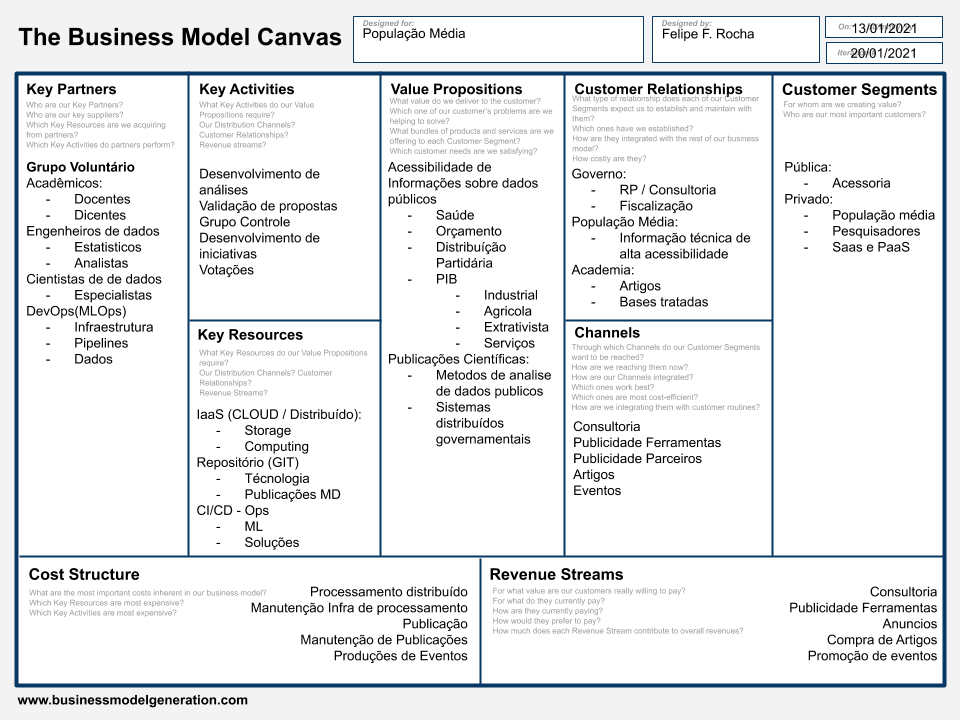
\includegraphics[height=4cm,keepaspectratio=true]{docs/BM.png}
    \caption{Business Model Canvas}
    \label{fig:BM}
    \centering
\end{figure}

Considerando fornecedores e clientes como entidades, detalha se abaixo as duas entidades.
\subsection{Fornecedores}
Os fornecedores podem ser divididos em duas grandes classes, sendo elas:
\begin{itemize}
    \item serviços (Cloud / IaaS) - plataforma e infraestrutura de troca de informações.
    \item voluntários (profissionais) - Produção de conhecimento, plataformas e analises de dados
\end{itemize}

\subsection{Clientes}
Podem ser divididos em 2 grupos, sendo elas:
\begin{itemize}
    \item Público - Reconhecendo o valor do grupo e da produção de conhecimento, poderia solicitar analises para melhor entendimento das situações diversas do governo.
    \item Privado - Esse ainda poderia ser divíduo em outros grupos sendo:
    \begin{itemize}
    \item População - acompanhando as informações mais acessíveis produzidas pelo grupo
    \item Privado - Pesquisadores interessados nas propostas e métodos, bases geradas e artigos
    \end{itemize}
\end{itemize}
Considerando as entidades citadas acima podemos fazer a análise de viabilidade em três pontos, econômica, social e ambiental.
\begin{itemize}
    \item Econômica - O projeto tem mão de obra voluntária e é aberto a comunidade, e além disso utiliza de tecnologias gratuitas e open source no desenvolvimento. Os maiores custos estão envolvidos em hospedar a solução em um ambiente Cloud e que pode ser substituído por um ambiente local se necessário. Dessa forma o projeto é viável economicamente.
    \item Social - Um dos objetivos do projeto é disponibilizar informação de forma acessível e simples para a população leiga e também disponibilizar uma metodologia para desenvolvimento de projetos similares com temáticas que agreguem informação para a sociedade. Dessa forma, fica claro que o projeto possui viabilidade social com impactos sociais bem definidos. 
    \item Ambiental - O projeto não possui uma ligação direta com questões ambientais, por isso a viabilidade ambiental é irrelevante neste caso.
\end{itemize}


% \write18{wget https://upload.wikimedia.org/wikipedia/commons/4/47/PNG_transparency_demonstration_1.png}
% \includegraphics{PNG_transparency_demonstration_1.png}

% \subsection{Artigos}


% \section{Descrição do }


% \section{Resultados e análise}

% \begin{gather}
%  y_{ij~visitados}
%  =
% \begin{bmatrix}
% 0 & 0 & 0 & 1 & 0\\
% 1 & 0 & 0 & 0 & 0\\
% 0 & 0 & 0 & 0 & 0\\
% 0 & 1 & 0 & 0 & 0\\
% 0 & 0 & 0 & 0 & 0
%   \end{bmatrix}
% \end{gather}


% \section{Conclusão}


% Embora o


% \appendices
% \section{Algorítimo de testes}

% Anexo I - "ModeloOtimizaçãoLinearSimples.R"
% %\\Anexo II - "Tabela de testes.xlsx"

% \ifCLASSOPTIONcaptionsoff
%   \newpage
% \fi

\printbibliography

\end{document}
